\documentclass{article}

\begin{document}

\setlength{\parindent}{6ex}

\begin{figure}
    \centering
    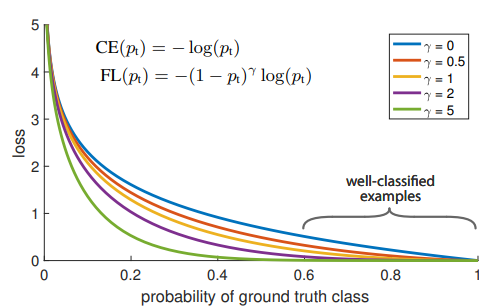
\includegraphics[width=0.75\textwidth]{focalloss}
    \caption{Focal Loss \cite{flretnetcite}. The effect of 
    gamma can be observed. The contribution of well-classified 
    examples to loss function reduces when gamma increases. 
    Detectors are more focused on hard, misclassified examples. Thus, 
    the accuracy of detectors are increased since they learn less 
    from the well-classified examples, yet, more from the hard, 
    misclassified examples.}
    \label{fig:focalloss1}
\end{figure}

\indent

In general, two-stage detectors have better accuracy than one-stage 
detectors. This article aims to find out why this is the case. 
Two-stage detectors are applied to a sparse set of candidate object 
locations. However, one-stage detectors are applied over a dense sampling 
of possible object locations. Then, the obtained result is the 
foreground-background class imbalance in the training of dense detectors.
The improved solution to this problem is called focal loss (Fig. 
\ref{fig:focalloss1}) which is introduced by this article. \par

Focal loss \cite{flretnetcite} is the reshaped version of cross-entropy loss. The aim of 
this change in cross-entropy is to down-weights the loss calculated for 
well-classified examples. Thus, the detector is trained on a sparse set of 
hard examples. Also, the class imbalance is handled by focal loss and 
sampling examples are not required since well-learned examples do not 
overwhelm loss during training. You can see the change in the loss by looking at 
figure \ref{fig:focalloss1}. When $\gamma$ equals to zero, the focal loss is 
equivalent to cross-entropy loss. For higher values of $\gamma$, the 
convergence of loss values changes as in the figure \ref{fig:focalloss1}. 
The best-performing $\gamma$ value equals to two according to the article.

\begin{figure}
    \centering
    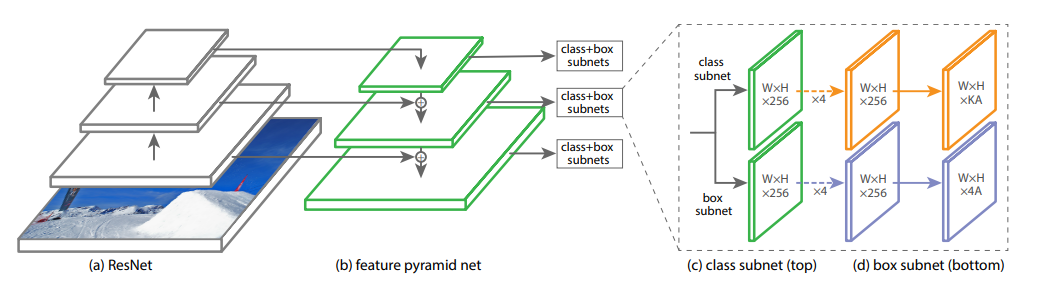
\includegraphics[width=\textwidth]{models/retinanet}
    \caption{Network of RetinaNet \cite{flretnetcite}. Feature pyramid network 
    is used after ResNet to generate a fine-grained, multi-scale convolutional 
    feature pyramid. Then, two subnetworks are attached after RetinaNet in which 
    one for classifying anchor boxes and the other one for regressing final 
    bounding boxes from anchor boxes. }
    \label{fig:retinanet1}
\end{figure}
\indent

RetinaNet \cite{flretnetcite} is designed to show the effectiveness of Focal Loss. As you 
can see in figure \ref{fig:retinanet1}, RetinaNet uses ResNet as its 
backbone network and FPN to obtain a multi-scale convolutional feature 
pyramid. Then, two subnetworks are used to obtain detection results. 
One of them is used to classify anchor boxes to obtain the classification of 
objects in anchor boxes and the other one is used to regress bounding 
boxes from anchors in which the aim is to obtain ground-truth bounding 
boxes.
\end{document}